\section[Modélisation ensembliste]{Modélisation ensembliste}
\begin{frame}{Modélisation ensembliste (1/2)}
	\begin{itemize}
	    \item Approche qui date du début des années 2010
        \item Focus sur des objets métiers
        \item Séparation des données statiques et dynamiques
        \item Schéma évolutif
        \item Bonnes performances grâce aux optimiseurs de requêtes modernes (élimination de tables/jointures)
	\end{itemize}
\end{frame}
\begin{frame}{Modélisation ensembliste (2/2)}
	Les deux approches qui se dégagent dans cette mouvance sont:
	\begin{minipage}{0.4\linewidth}
	   \hspace{10cm}
       \begin{figure}
            
\includegraphics[scale=0.2]{figures/vault.png}
            \caption{Data vaults}
		\end{figure}
	\end{minipage}
	\hspace{1cm}
    \begin{minipage}{0.4\linewidth}	
    \hspace{10cm}
        \begin{figure}
            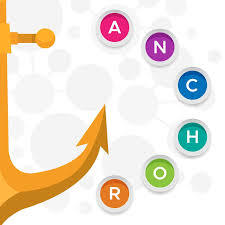
\includegraphics[scale=0.33]{figures/anchor.jpg}
            \caption{Anchor modeling}
		\end{figure}
    \end{minipage}
\end{frame}
\subsection{Data Vaults}
\begin{frame}{Data vaults (1/2)}
\begin{itemize}
    \item Dan Linstedt
    \item Création : 1990
    \item Domaine public : 2000
    \item Répondre aux besoins de l’industrie
    \item Défini au niveau logique relationnel
\end{itemize}
\vspace{0.1cm}
\textbf{=> }Permet la construction incrémentale du schéma à moindre coût \\
\end{frame}
\begin{frame}{Data vaults (2/2)}
Un data vault est composé des éléments principaux : 
\begin{itemize}
    \item Centre (Hub) est une entité de base qui représente un concept métier. Il contient principalement une clé (business key)
    \item Lien (Link) matérialise une association entre deux centres ou plus.
\end{itemize}
\centering
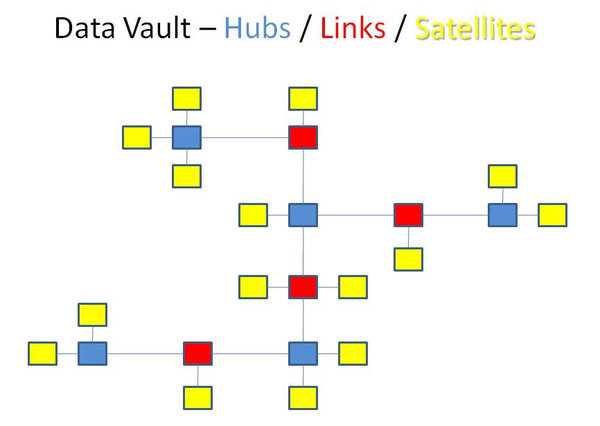
\includegraphics[scale=0.3]{figures/vault2.jpeg}
\end{frame}
\subsection{Anchor Modeling}
\begin{frame}{Anchor Modeling}
\begin{itemize}
    \item Olle Regardt, Lars Rönnbäck
    \item Premier test : 2004
    \item Publication : 2007
\end{itemize}
\centering
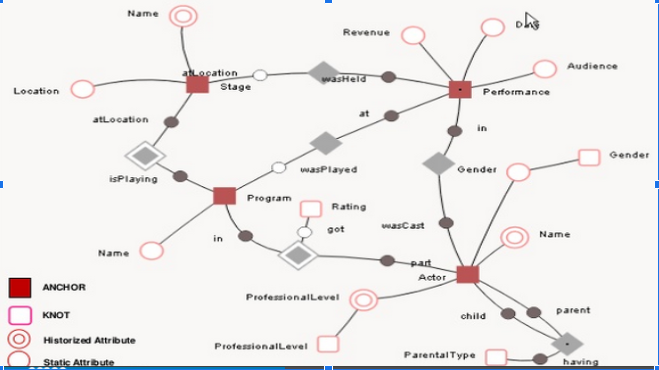
\includegraphics[scale=0.55]{figures/anchor2.PNG}
\end{frame}